\chapteropener{Probabilistic}{orangehard}{orangeaccent}{%
In this chapter, we check whether a model's probabilities match observed outcomes and estimate its performance before new labels
arrive. A loan model, for example, predicts repayment when someone applies, but we may wait months to learn whether they repay.
Earlier predictions and their outcomes can help us estimate performance during that wait.

Those earlier examples form a labeled \emph{reference dataset}. The estimator learns from their known outcomes, then estimates
performance for each new batch of predictions before its labels arrive. Each batch forms a \emph{chunk}
in the figures. We keep the reference examples separate from the monitored model's training data and validate the estimator on
held-out data.

Expected Calibration Error (ECE) measures \emph{calibration}: how well predicted probabilities agree with observed outcomes.
Two classification methods, CBPE and PAPE, then use calibrated probabilities to estimate metrics such as accuracy and F1.
For regression, Direct Loss Estimation (DLE) learns to predict the model's error.

These estimates can track changes in the input mix, or \emph{covariate shift}, but they assume the relationship between inputs
and outcomes stays the same. If that relationship changes, we have \emph{concept drift}. Once labels arrive, Reverse Concept
Drift (RCD) helps us estimate its effect on performance.}{In this chapter}

% ---------- Decision map ----------
\begin{decisionmap}{orangehard}{orangeaccent}{Which metric?}{Follow the branches to a method. The number next to it is its page.}
\maproot{Have the labels arrived?}
\begin{forest} dmap, large
[, coordinate, l sep=0pt
  [{\dl{yes: how much is concept drift?}{\mref{RCD}{sec:rcd}}}]
  [{\dm{no, and it is a classifier}{Are the reference probabilities calibrated?}}
    [{\dl{check that first}{\mref{ECE}{sec:ece}}}]
    [{\dl{calibration still holds in production}{\mref{CBPE}{sec:cbpe}}}]
    [{\dl{input mix changed; reference covers it}{\mref{PAPE}{sec:pape}}}]
  ]
  [{\dl{no, and it is a regressor}{\mref{DLE}{sec:dle}}}]
]
\end{forest}
\end{decisionmap}


% ---------- Expected Calibration Error ----------
\clearpage
\thispagestyle{probabilisticstyle}
\section{ECE}\label{sec:ece}
\subsection{Expected Calibration Error}

% reference:
% Naeini, Cooper, Hauskrecht (2015) — Obtaining Well Calibrated Probabilities Using Bayesian Binning
% Guo, Pleiss, Sun, Weinberger (2017) — On Calibration of Modern Neural Networks (temperature scaling)
% Murphy (1973) — decomposition of the Brier score

Expected Calibration Error measures the gap between a classifier's confidence and how often its predictions are correct. Here,
confidence means the probability assigned to the predicted class. If predictions made with about $80\%$ confidence are correct
only $70\%$ of the time, the model is overconfident in that range. ECE groups predictions into confidence bins and averages these
gaps, giving more weight to bins with more predictions.

% equation
\begin{center}
    \tikz{
        \node[inner sep=2pt, font=\Large] (a) {
            {
                $\displaystyle
                \text{ECE} = \sum_{b=1}^{B} \frac{{\color{nmlred}|B_b|}}{{\color{nmlred}n}} \,\Big|\, {\color{nmlcyan}\text{acc}}(B_b) - {\color{nmlpurple}\text{conf}}(B_b) \,\Big|
                $
            }
        };
        \path[room for labels] ([yshift=0.25cm]a.north) ([yshift=-0.12cm]a.south);
        \draw[overlay,-latex,nmlred, semithick] ($(a.south)+(-1.28,0.36)$) to[bend left=15] node[pos=1, left] {share of bin $b$} +(-1.00,-0.51);
        \draw[overlay,-latex,nmlcyan, semithick] ($(a.north)+(-0.09,-0.69)$) to[bend right=15] node[pos=1, left] {observed accuracy} +(-1.00,0.95);
        \draw[overlay,-latex,nmlpurple, semithick] ($(a.north)+(2.44,-0.58)$) to node[pos=1, above] {mean confidence} +(0.00,0.30);
    }
\end{center}

ECE ranges from $0$ to $1$: $0.08$ means an average gap of eight percentage points across the bins. There is no universal cutoff
for good calibration; the result depends on the bin boundaries, sample size, and which predictions are grouped together.

\textbf{When to use ECE?}

Use ECE on held-out labeled data when confidence affects decisions or to compare calibration methods. For a loan's repayment
probability, or for CBPE, check positive-class calibration too: group by the probability of repayment and compare it with the fraction who repay.
The confidence-based ECE shown here can hide differences between classes.

\enlargethispage{\baselineskip}
\coloredboxes{
\item Summarizes calibration in probability units, so comparisons using the same data and bins are easy to interpret.
\item A reliability diagram shows which confidence ranges are overconfident or underconfident, helping explain the overall score.
}
{
\item Wide bins can hide errors that cancel out; narrow bins may contain too few examples. Report the binning scheme and inspect counts.
\item Low ECE does not imply useful predictions. Always predicting the class proportions can be calibrated while failing to distinguish individual cases.
}

\clearpage

\thispagestyle{customstyle}

\begin{center}
    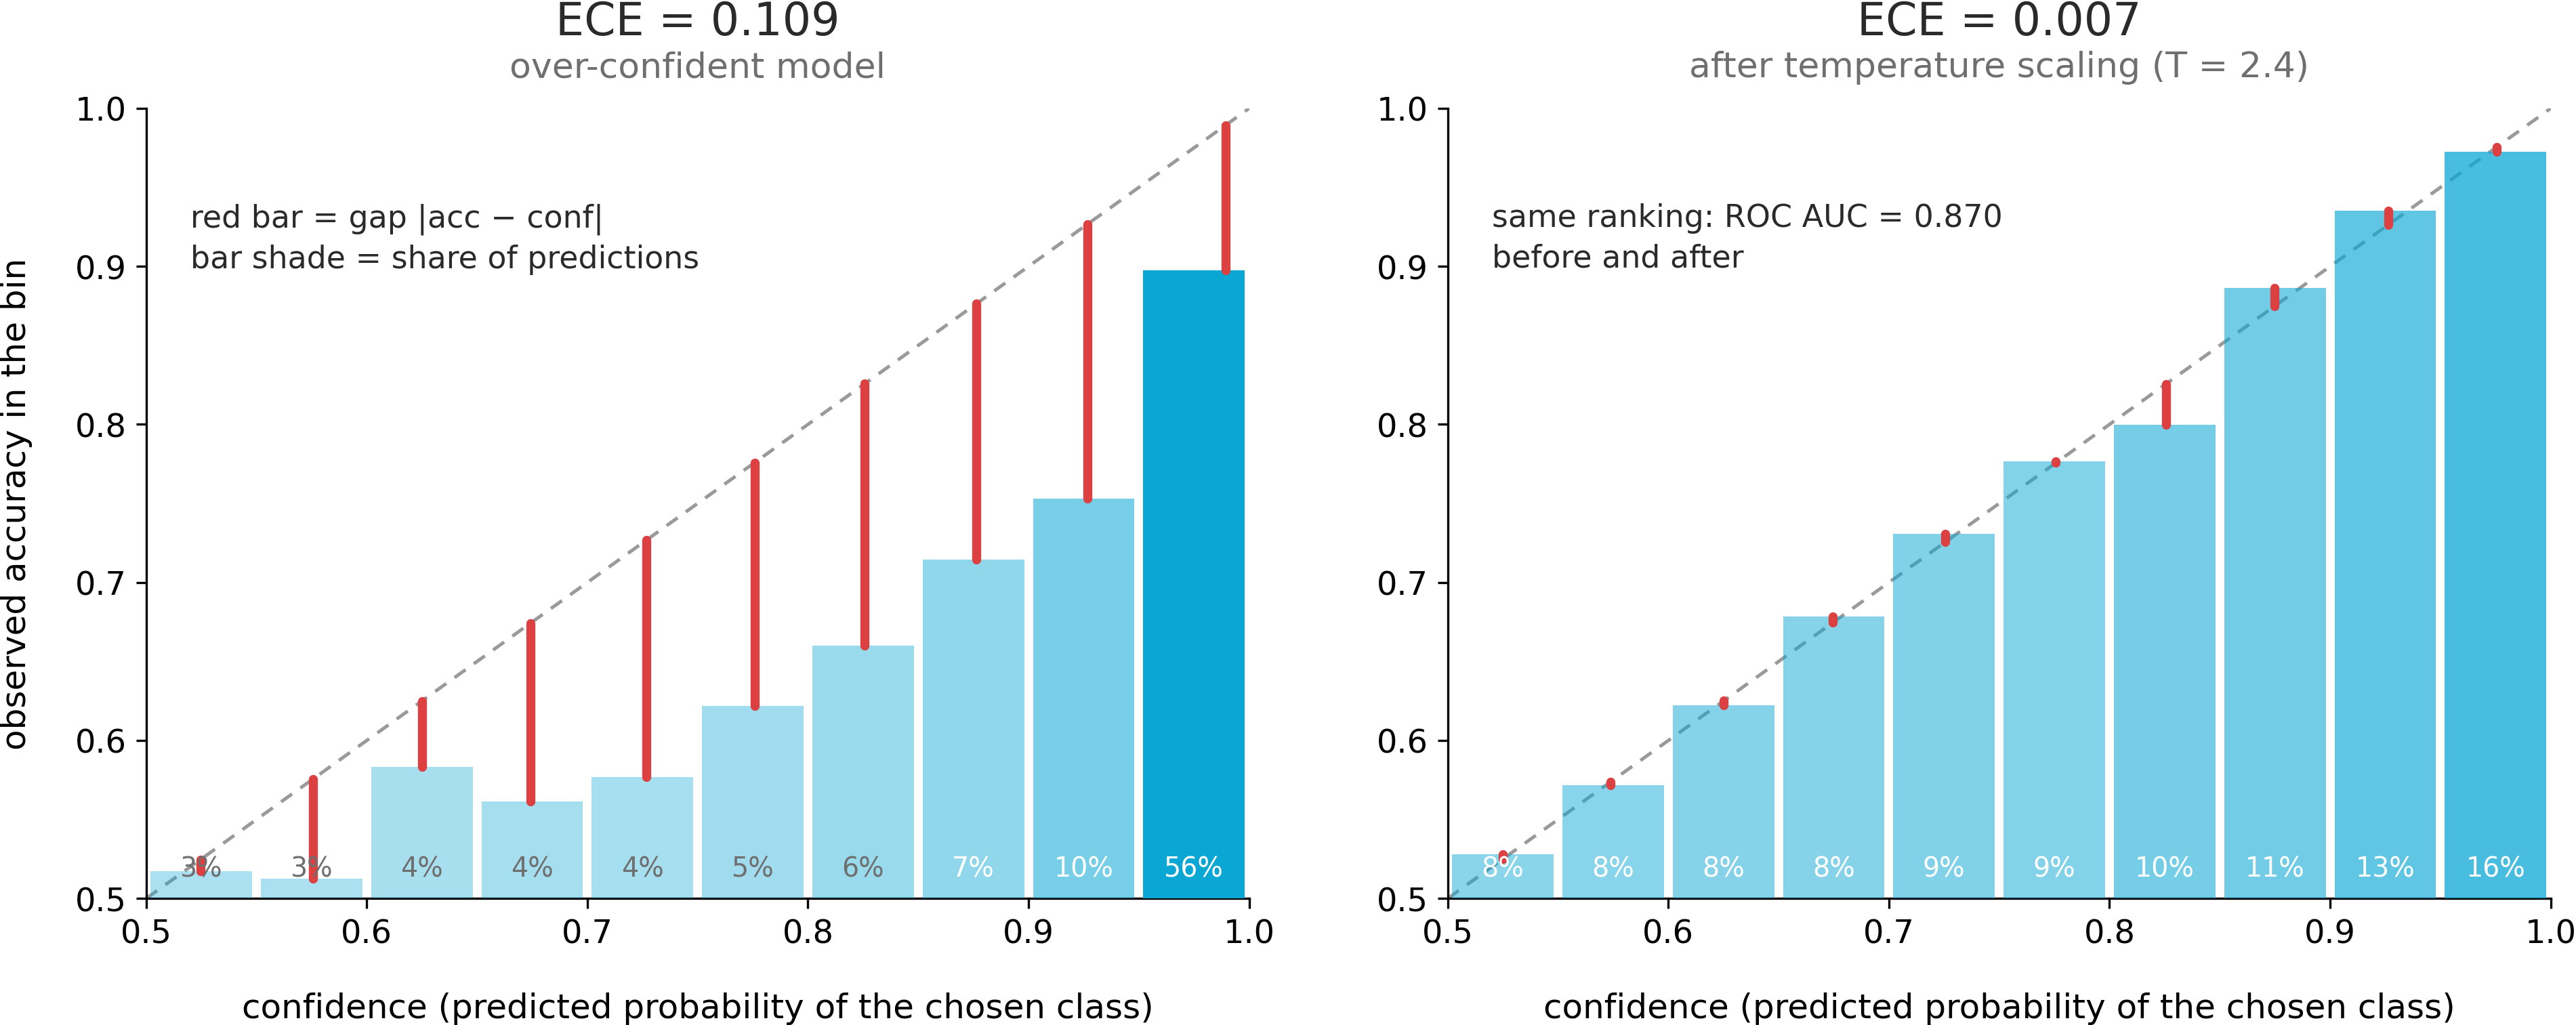
\includegraphics[width=\textwidth]{figures/ECE_reliability.png}
\end{center}

\textbf{Figure. ECE.} Reliability diagrams for a simulated binary classifier before and after temperature scaling, which adjusts
confidence by dividing the model's raw scores (logits) by a positive value $T$. Each bar is a confidence bin: its
height is the observed accuracy, its shade the share of predictions, and the red segment the gap to the diagonal.
\underline{Left:} the model puts $55\%$ of its predictions in the top bin at a mean confidence of $0.99$ and is right $90\%$ of
the time there; the weighted gaps sum to $\text{ECE} = 0.110$. \underline{Right:} with $T = 2.5$, the bars move closer to the
diagonal and ECE falls to $0.007$. ROC AUC stays at $0.867$ because the ranking is unchanged in this binary example.

\orangebox{Did you know that...}
{DeGroot and Fienberg ($1983$) separated the Brier score into calibration and refinement terms. Calibration describes whether
probabilities match outcome frequencies; refinement describes how well the forecasts separate cases with different outcome rates.
A model that gives everyone the overall event rate can be calibrated while offering no such separation. Temperature scaling
illustrates another distinction: it preserves the predicted class in both binary and multiclass classification, but only in the
binary case does it necessarily preserve the ranking of probabilities across examples, and hence ROC AUC.}

\textbf{Other related metrics}

Brier score and log loss evaluate the probabilities as a whole, while ROC AUC measures ranking. Log loss can improve without
changing either ROC AUC or binned ECE, so read them together before explaining a change. Calibration within Groups
(Bias \& Fairness chapter) can reveal errors hidden by pooling groups; CBPE additionally needs calibration to hold in production.

% ---------- CBPE ----------
\clearpage
\thispagestyle{probabilisticstyle}
\section{CBPE}\label{sec:cbpe}
\subsection{Confidence-Based Performance Estimation}

% reference:
% https://nannyml.readthedocs.io/en/stable/how_it_works/performance_estimation.html#confidence-based-performance-estimation-cbpe
% https://arxiv.org/abs/2505.05295 (Kivimäki, Białek, Kuberski, Nurminen, 2025)

CBPE estimates a classifier's performance from probabilities before labels arrive. A fraud model can therefore be monitored
while chargebacks are still pending. Here, $c_j$ is the calibrated probability of fraud and $\hat{y}_j$ the predicted label.
A transaction flagged as fraud with $c_j=0.9$ contributes $0.9$ to expected
true positives and $0.1$ to expected false positives.

% equation
\begin{center}
    \tikz{
        \node[inner sep=2pt, font=\Large] (a) {
            {
                $\displaystyle
                \widehat{\text{TP}} = \sum_{j} {\color{nmlpurple}c_j}\, \mathds{1}[{\color{nmlpurple}\hat{y}_j} = 1], \qquad
                \widehat{\text{FP}} = \sum_{j} (1 - {\color{nmlpurple}c_j})\, \mathds{1}[{\color{nmlpurple}\hat{y}_j} = 1]
                $
            }
        };
        \node[below=0.12cm of a, inner sep=2pt, font=\large] (b) {
            $\displaystyle
            \widehat{\text{FN}} = \sum_{j} {\color{nmlpurple}c_j}\, \mathds{1}[{\color{nmlpurple}\hat{y}_j} = 0], \qquad
            \widehat{\text{TN}} = \sum_{j} (1 - {\color{nmlpurple}c_j})\, \mathds{1}[{\color{nmlpurple}\hat{y}_j} = 0]
            $
        };
        \draw[overlay,-latex,nmlpurple, semithick] ($(a.north)+(-2.50,-0.22)$) to node[pos=1, above] {calibrated probability} +(0.00,0.30);
        \draw[overlay,-latex,nmlpurple, semithick] ($(a.north)+(3.27,-0.36)$) to node[pos=1, above] {predicted label} +(0.00,0.43);
    }
\end{center}

The indicator $\mathds{1}$ selects the predictions with the stated label, and each sum runs over one production batch. An
unflagged transaction contributes $c_j$ to expected false negatives and $1-c_j$ to expected true negatives. Substituting these
counts into metric formulas gives expected accuracy and precision, and approximations for recall and F1.

\textbf{When to use CBPE?}

Use CBPE when labels are delayed and calibration is expected to hold in production. Fit the calibrator on labeled reference
predictions and validate the estimates on separate data. If a changing input mix disrupts calibration, consider PAPE; neither
method can reliably estimate performance for inputs absent from the reference data.

\enlargethispage{2\baselineskip}
\coloredboxes{
\item Estimates several metrics from one expected confusion matrix, without waiting for production labels.
\item Can follow performance changes caused by a new input mix when calibration still holds.
}
{
\item Misses concept drift when inputs stay the same: changed outcomes do not change the model's probabilities.
\item Estimated accuracy is at least $0.5$ if each label chooses the more likely class under the probabilities used.
}

\clearpage

\thispagestyle{customstyle}
\enlargethispage{\baselineskip}

\begin{center}
    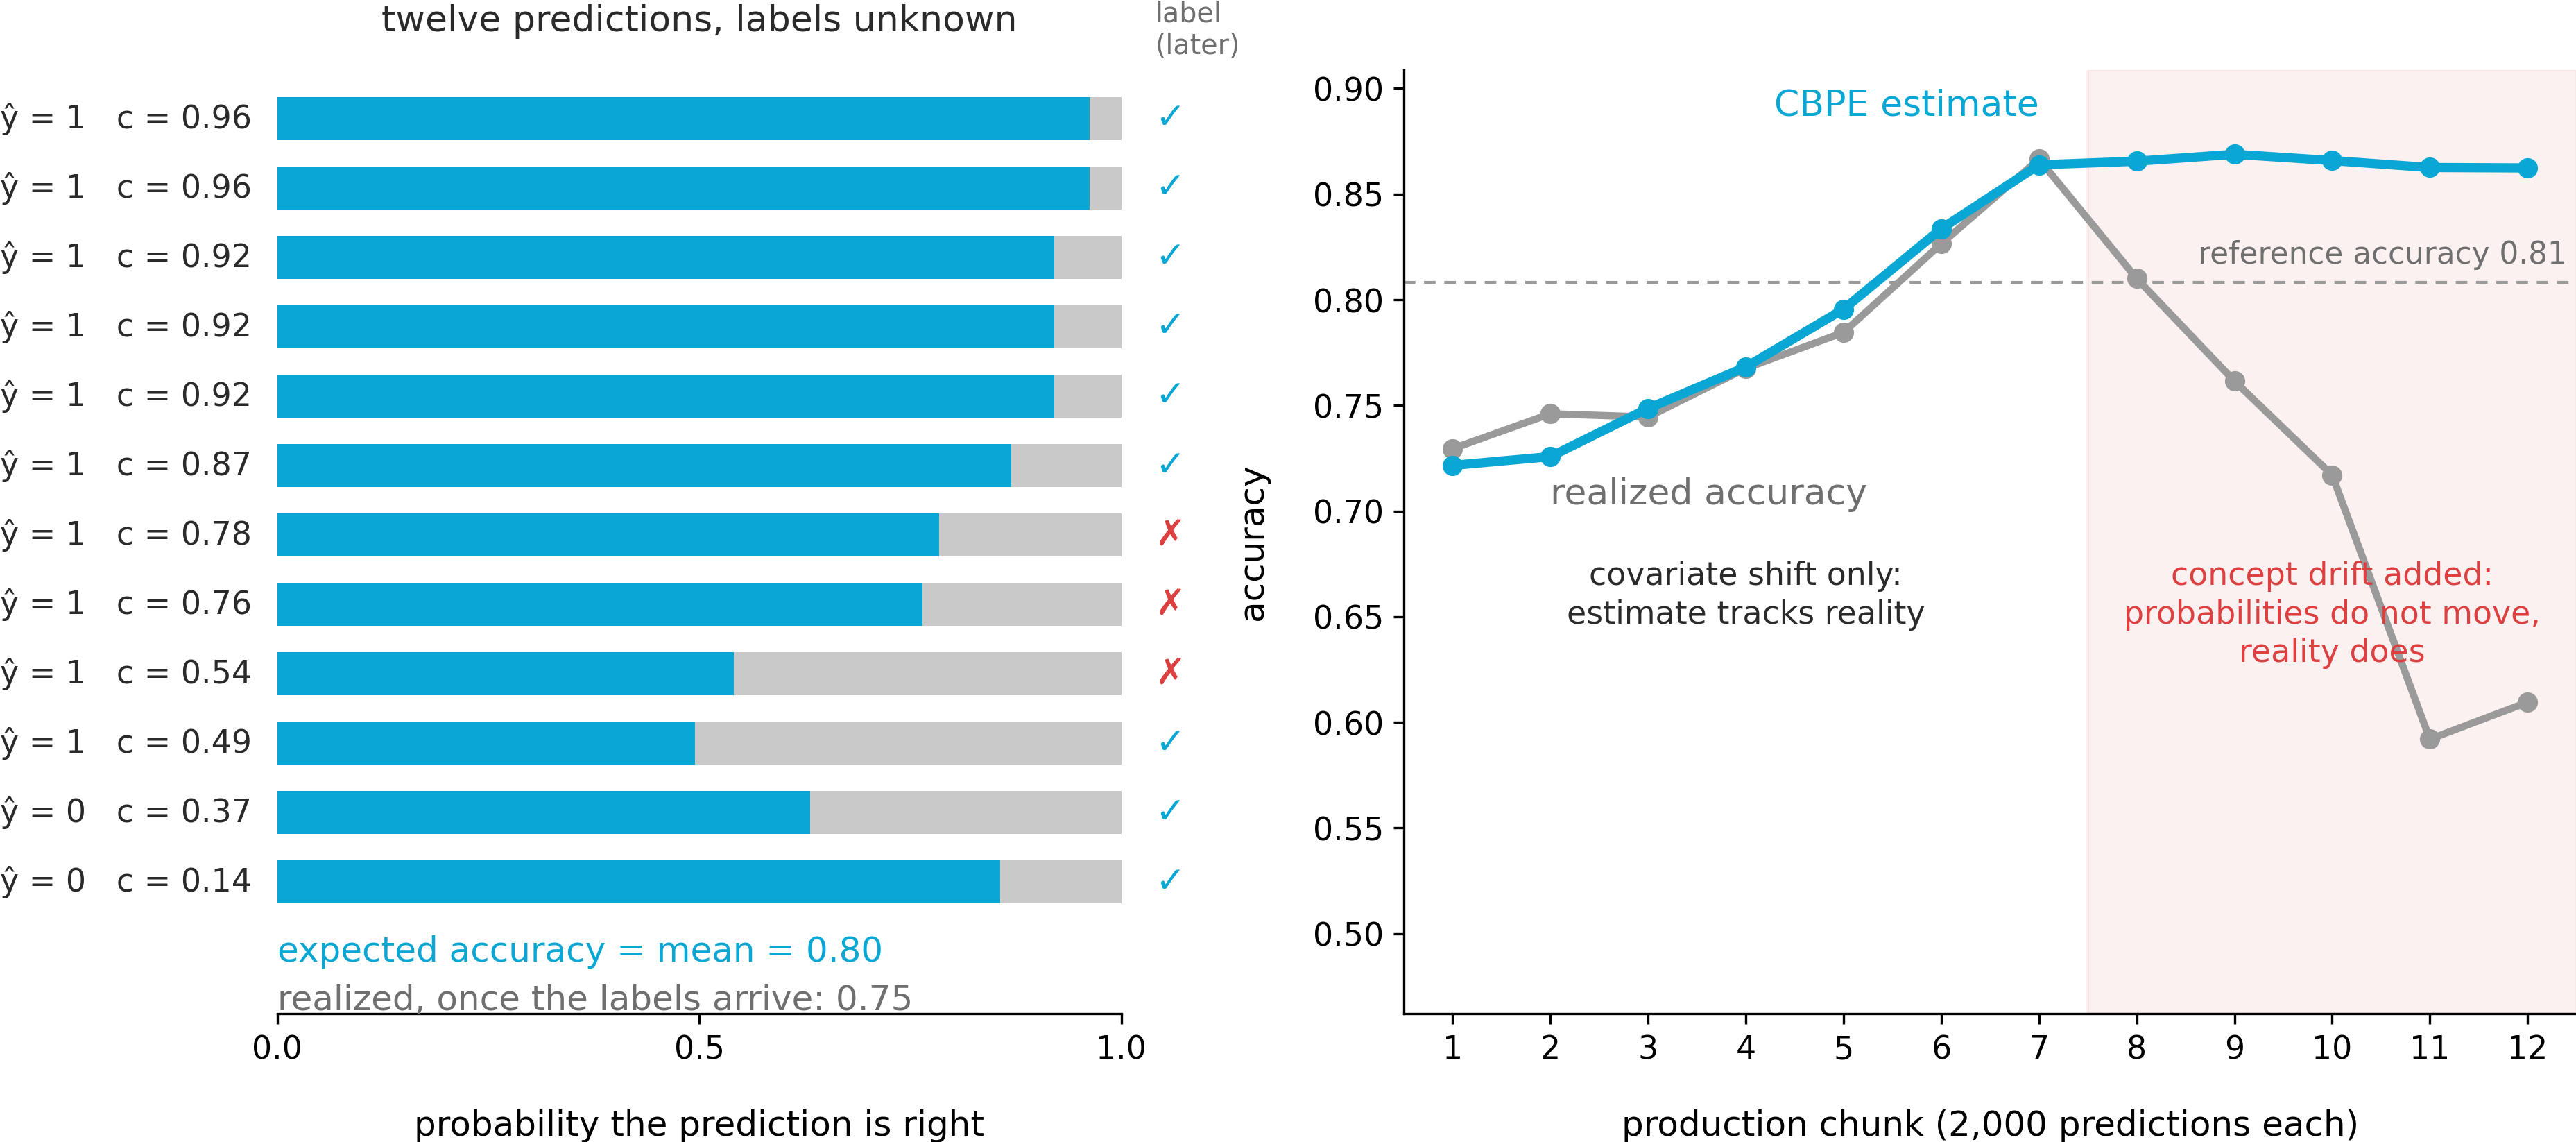
\includegraphics[width=\textwidth]{figures/CBPE_estimation.png}
\end{center}

\textbf{Figure. CBPE.} \underline{Left:} twelve production predictions with calibrated probabilities and no labels. Each bar is the
probability the prediction is right, $c$ for $\hat{y}=1$ and $1-c$ for $\hat{y}=0$; their mean, $0.77$, is the expected accuracy. The
labels that arrive later make nine of twelve right, $0.75$. \underline{Right:} twelve simulated chunks of $2{,}000$ predictions.
Accuracy rises as the input mix changes in chunks $1$--$7$. From chunk $8$, the input--outcome relationship changes too: accuracy
falls to $0.60$, while the estimate stays near $0.86$. The illustrative band follows the estimate at $\pm 3$ standard deviations
of reference-chunk accuracy; it is neither a validated uncertainty interval nor a fixed alert threshold.

\orangebox{Did you know that...}
{Even a sound estimate need not equal the accuracy measured when labels arrive. For $2{,}000$ independent predictions, each with
an $80\%$ chance of being correct, the standard error of accuracy is $\sqrt{0.8(1-0.8)/2{,}000}\approx0.009$, almost one percentage
point. Uncertainty intervals account for variation around an estimate, while historical alert thresholds flag changes from past
performance. To judge a gap, consider both sampling variation and estimation error.}

\textbf{Other related metrics}

Low reference ECE does not bound production error. PAPE adjusts calibration for a changed input mix, but its estimates also need
validation. When labels arrive, investigate gaps between estimated and measured performance; RCD can help assess concept drift,
while estimator error and sampling variation may also contribute.

% ---------- PAPE ----------
\clearpage
\thispagestyle{probabilisticstyle}
\section{PAPE}\label{sec:pape}
\subsection{Probabilistic Adaptive Performance Estimation}

% reference:
% https://docs.nannyml.com/cloud/model-monitoring/how-it-works/probabilistic-adaptive-performance-estimation-pape
% https://arxiv.org/abs/2401.08348 — Estimating Model Performance Under Covariate Shift Without Labels

PAPE estimates classification performance by adapting calibration to the production input mix. Suppose a loan model assigns
$80\%$ repayment probability to two equally sized applicant groups, but their repayment rates are $90\%$ and $70\%$. The combined
rate is $80\%$, so calibration looks right. If the first group becomes more common, the combined rate rises even though neither
group's behavior changed. PAPE gives reference examples from that group more weight when refitting the calibrator.

% equation
\begin{center}
    \tikz{
        \node[inner sep=2pt, font=\Large] (a) {
            {
                $\displaystyle
                \hat{w}(x) = \frac{{\color{nmlred}n_{\text{ref}}}}{{\color{nmlred}n_{\text{prod}}}} \cdot \frac{{\color{nmlpurple}\hat{p}}(z = 1 \mid x)}{{\color{nmlpurple}\hat{p}}(z = 0 \mid x)}
                $
            }
        };
        \path[room for labels] ([yshift=0.13cm]a.north) ([yshift=-0.18cm]a.south);
        \draw[overlay,-latex,nmlred, semithick] ($(a.north)+(-0.60,-0.18)$) to[bend right=15] node[pos=1, left] {sample sizes} +(-1.00,0.30);
        \draw[overlay,-latex,nmlpurple, semithick] ($(a.south)+(0.48,0.09)$) to[bend left=15] node[pos=1, left] {domain classifier} +(-1.00,-0.30);
    }
\end{center}

$\hat{w}(x)$ estimates the density ratio $p_{\text{prod}}(x)/p_{\text{ref}}(x)$ from a classifier trained to tell production
($z=1$) from reference ($z=0$): inputs twice as common get weight $2$. The calibrator is fit on reference labels with these weights,
applied to production scores, and the confusion matrix is built as in CBPE.

\textbf{When to use PAPE?}

Use PAPE when a changed customer mix may have disrupted calibration, provided the reference data covers the inputs seen in
production. Check that enough reference examples support the new mix. Weighting cannot supply missing examples or reveal
concept drift without new labels.

\enlargethispage{\baselineskip}
\coloredboxes{
\item Uses production inputs to adjust reference calibration, so it can follow changes that a fixed calibrator misses.
\item Recomputes weights for each chunk, allowing the calibration adjustment to change as the customer mix changes.
}
{
\item Cannot extrapolate: the density ratio is undefined where production has inputs with no reference support.
\item Inaccurate weights distort calibration. If a few reference examples carry most of the weight, the estimate can be unstable even with many rows.
}

\clearpage

\thispagestyle{customstyle}

\begin{center}
    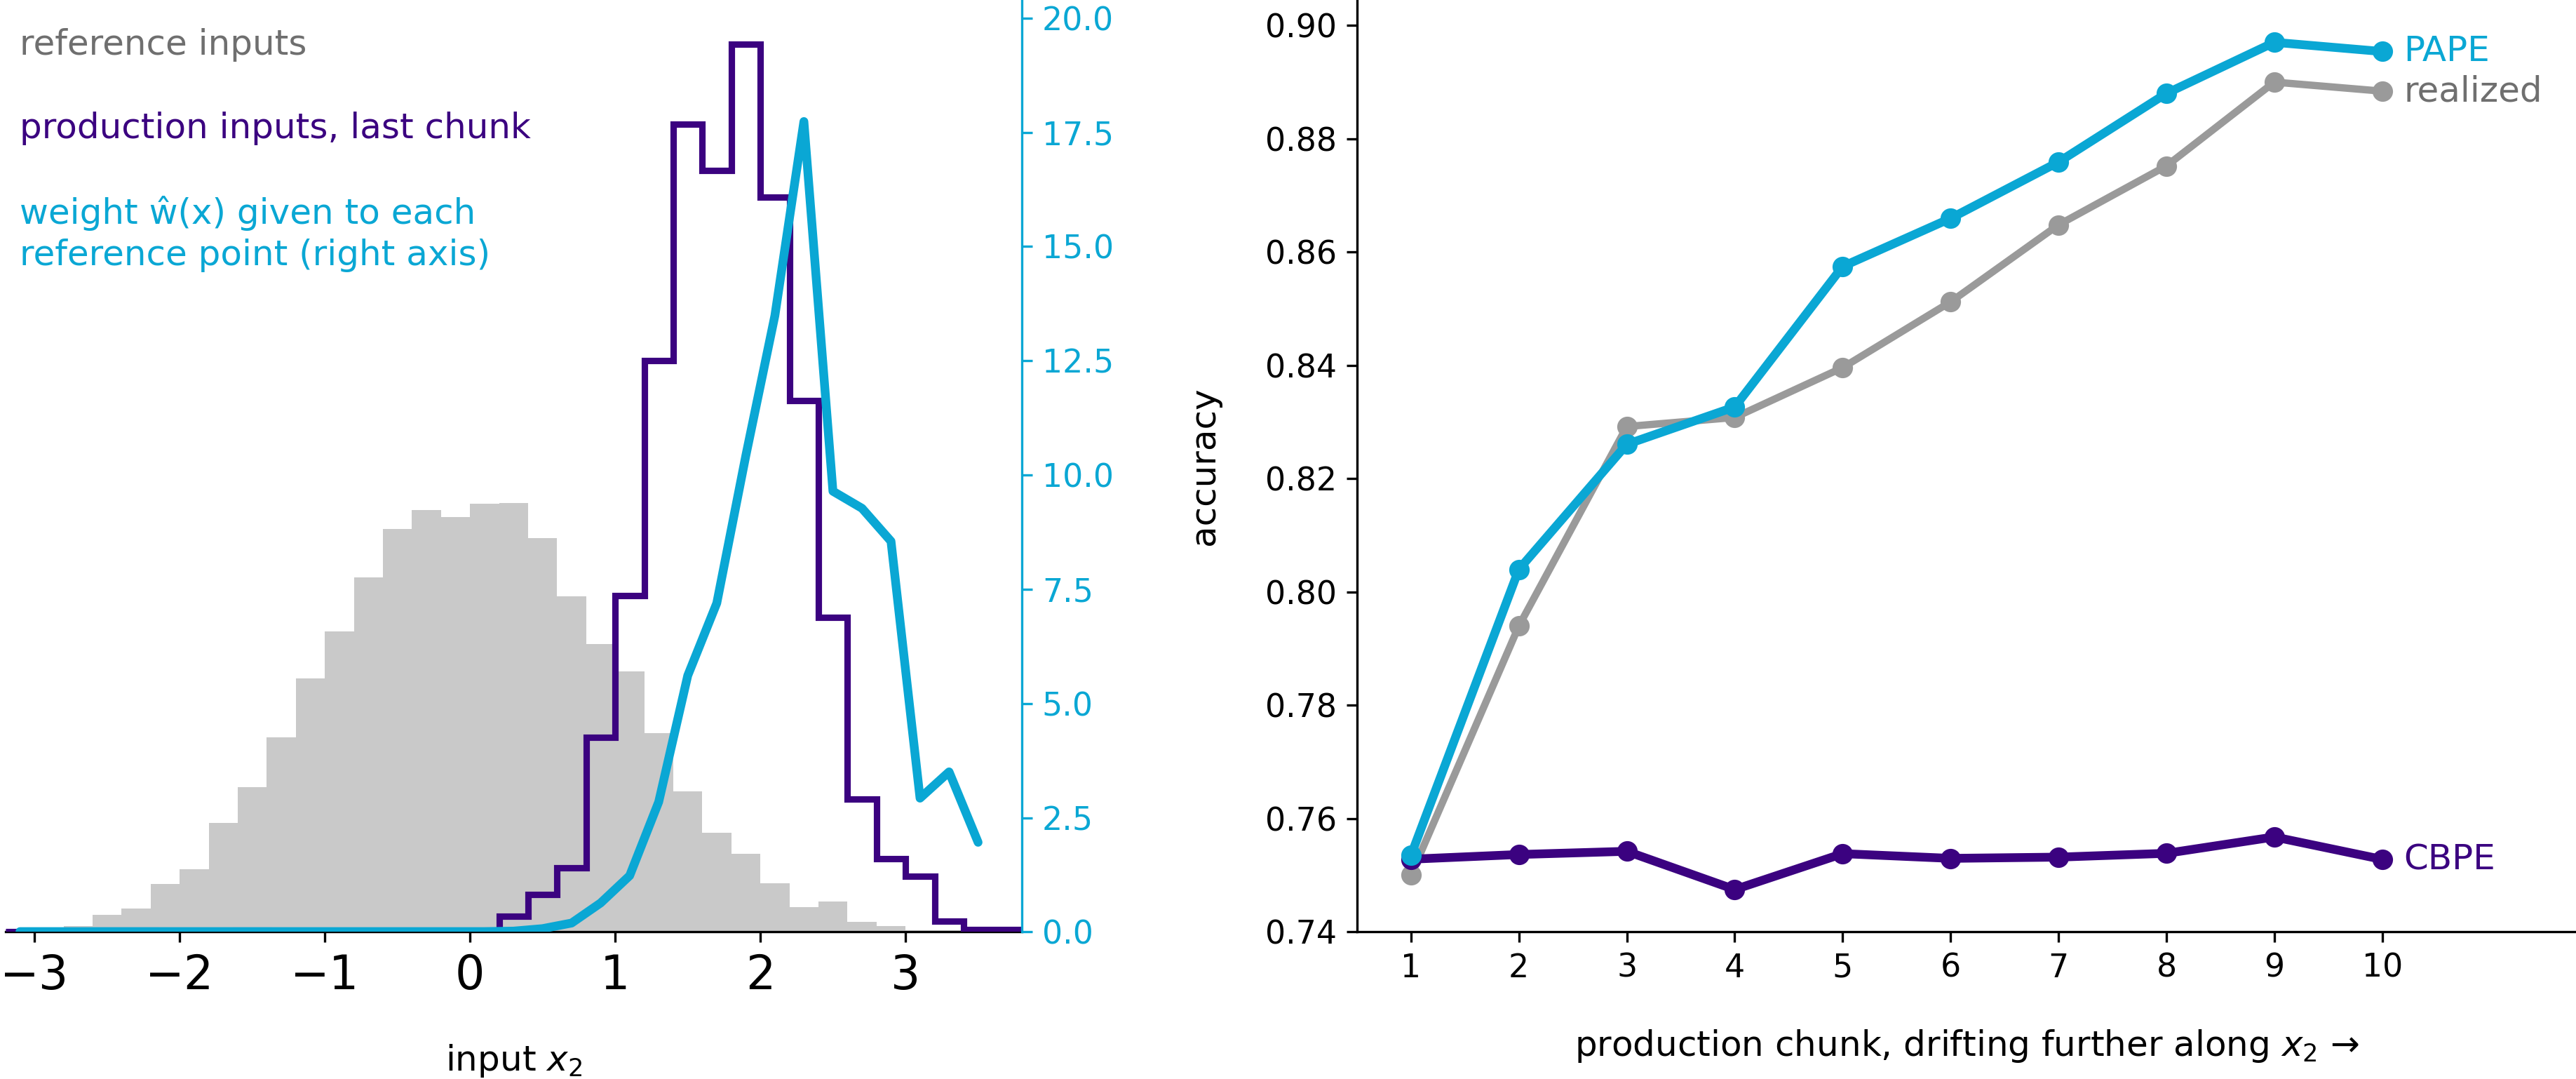
\includegraphics[width=\textwidth]{figures/PAPE_reweighting.png}
\end{center}

\textbf{Figure. PAPE.} A simulated classifier whose calibration varies with an artificial input, $x_2$.
\underline{Left:} the reference (gray) and final production chunk (purple) have different input distributions. The curve shows
the mean weight assigned to reference points at each $x_2$, about $18$ near the production region and close to zero elsewhere.
\underline{Right:} CBPE uses the fixed reference calibration and stays near $0.75$ while realized accuracy climbs to
$0.89$; PAPE follows it with a mean absolute error of $0.009$ against CBPE's $0.089$.

\orangebox{Did you know that...}
{Importance weighting can estimate performance directly by giving more weight to errors on reference examples that resemble
production. PAPE instead uses those weights to fit a calibrator, then estimates performance from production predictions.
In Białek and colleagues' $2025$ benchmark, covering $959$ evaluation cases and $36{,}557$ production chunks from US census data,
PAPE had the lowest aggregate error for accuracy, F1, and ROC AUC among eight evaluated methods. That result supports the approach
in those experiments; it does not guarantee that weighting improves every estimate.}

\textbf{Other related metrics}

If CBPE and PAPE disagree, check whether production inputs are covered by the reference data and whether a few examples dominate
the weights. Compare both estimates with measured performance on labeled periods with similar shifts before choosing between them.
DLE estimates regression loss; RCD uses new labels to assess the effect of a changed input--outcome relationship.

% ---------- DLE ----------
\clearpage
\thispagestyle{probabilisticstyle}
\section{DLE}\label{sec:dle}
\subsection{Direct Loss Estimation}

% reference:
% https://nannyml.readthedocs.io/en/stable/how_it_works/performance_estimation.html#direct-loss-estimation-dle

Direct Loss Estimation estimates a regression model's performance by learning how large its errors tend to be for different
inputs. A demand forecast, for example, may be more accurate for staples than for promotions. DLE trains a second model on
reference errors, then averages its predicted losses over each production batch. In NannyML's terminology, this loss model is
the \emph{nanny}, and the monitored model is the \emph{child}.

% equation
\begin{center}
    \tikz{
        \node[inner sep=2pt, font=\Large] (a) {
            {
                $\displaystyle
                \widehat{\text{MAE}} = \frac{1}{{\color{nmlred}n}} \sum_{j=1}^{n} {\color{nmlpurple}h}\big({\color{nmlcyan}x_j},\, {\color{nmlpurple}f(x_j)}\big)
                $
            }
        };
        \path[room for labels] ([yshift=0.19cm]a.north) ([yshift=-0.00cm]a.south);
        \draw[overlay,-latex,nmlred, semithick] ($(a.south)+(-0.93,0.42)$) to[bend left=15] node[pos=1, left] {production size} +(-1.00,-0.30);
        \draw[overlay,-latex,nmlpurple, semithick] ($(a.north)+(0.28,-0.52)$) to[bend right=15] node[pos=1, left] {nanny model} +(-1.00,0.72);
        \draw[overlay,-latex,nmlcyan, semithick] ($(a.south)+(1.05,0.63)$) to[bend right=15] node[pos=1, right] {input} +(1.00,-0.30);
        \draw[overlay,-latex,nmlpurple, semithick] ($(a.north)+(2.45,-0.51)$) to node[pos=1, above] {child's prediction} +(0.00,0.33);
    }
\end{center}

For MAE, train $h$ to predict $|y-f(x)|$ from the inputs and the monitored model's prediction $f(x)$. These errors must come from
data that $f$ did not train on. For MSE, predict squared errors instead; for RMSE, take the square root after averaging them.
Validate $h$'s estimates on separate labeled data before using them for monitoring.

\textbf{When to use DLE?}

Use DLE when regression targets arrive late and the input mix changes. It is useful when expected loss varies predictably across
inputs, whether because of noise or systematic model errors. It cannot reliably handle a changed input--outcome relationship
or inputs outside the reference data.

\enlargethispage{\baselineskip}
\coloredboxes{
\item Estimates familiar regression metrics directly from losses, without having to model the full distribution of possible outcomes.
\item Error size can be easier to predict than the outcome itself: a promotion may have uncertain demand but consistently larger errors.
}
{
\item Assumes learned error patterns still hold. If errors grow for unchanged inputs, the loss model continues to predict the earlier error.
\item A second model needs training and validation. Noisy reference losses or a poorly fitted loss model can distort the performance estimate.
}

\clearpage

\thispagestyle{customstyle}

\begin{center}
    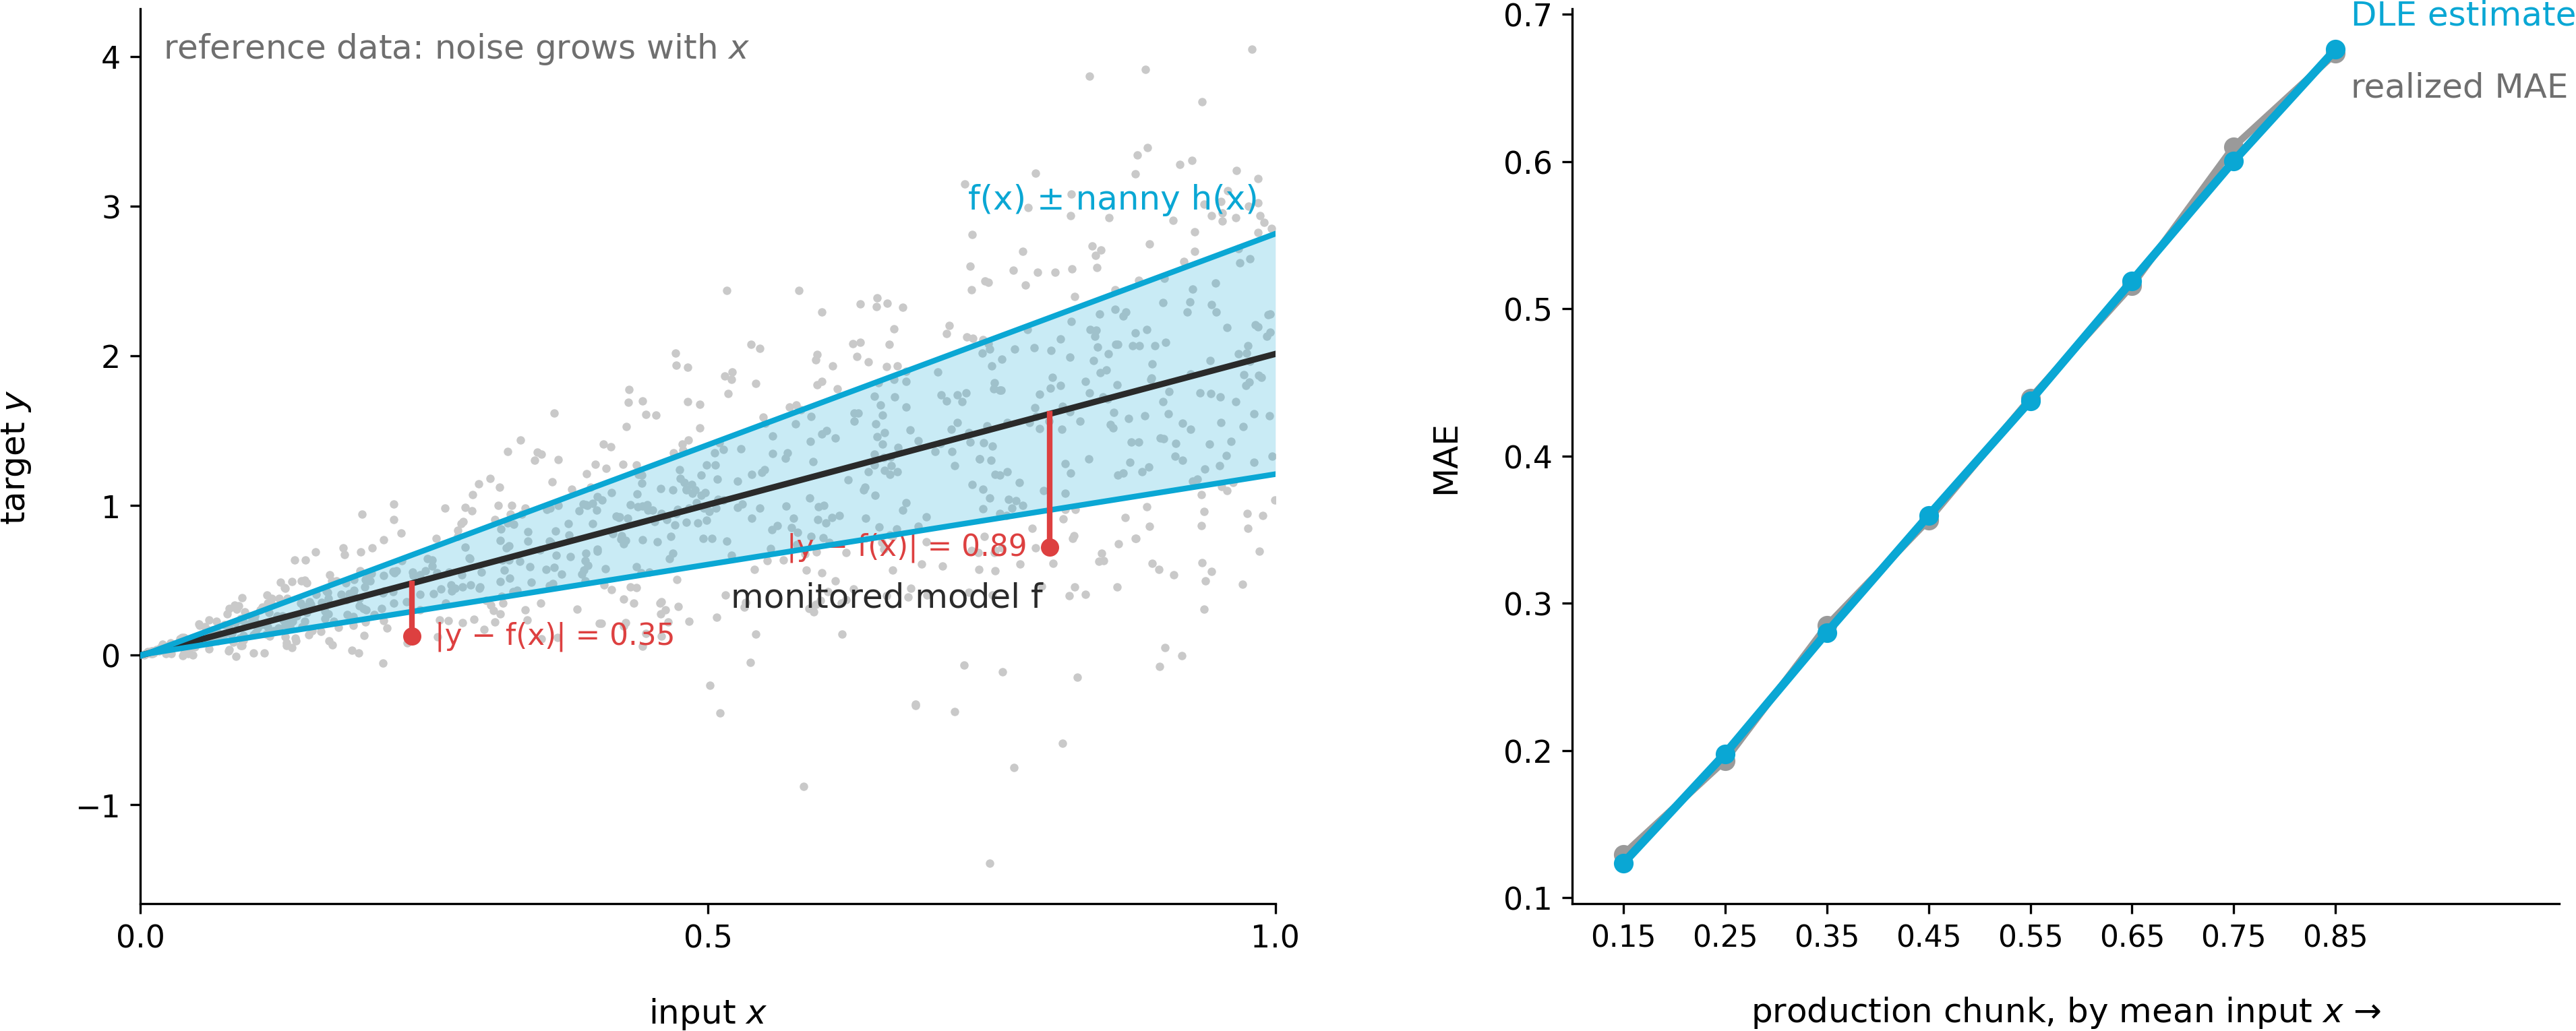
\includegraphics[width=\textwidth]{figures/DLE_nanny.png}
\end{center}

\textbf{Figure. DLE.} \underline{Left:} simulated data whose noise grows with the input, a linear prediction model $f$, and a
linear loss model $h$. The shaded band shows $f(x)\pm h(x)$: the prediction plus or minus the estimated mean absolute error.
It illustrates error size, with no stated coverage probability. Two absolute errors used to train $h$ are marked in red.
\underline{Right:} eight production chunks move toward the noisier region. Measured MAE rises from $0.13$ to $0.67$, and DLE
tracks it to within $0.01$ in this example.

\orangebox{Did you know that...}
{NannyML explored Bayesian models and conformalized quantile regression before adopting DLE. One attempt converted two predicted
quantiles into an outcome distribution by assuming it was normal, then calculated expected loss from that distribution.
Predicting the loss directly removed those intermediate steps. The normality assumption belonged to that particular conversion:
conformal prediction itself does not require normally distributed noise. Its usual coverage guarantee instead depends on
calibration and future examples being exchangeable, as they are under independent sampling from the same distribution.}

\textbf{Other related metrics}

CBPE and PAPE estimate classification performance; DLE learns the loss directly. When measured and estimated loss disagree,
check input changes, recent labeled errors, and the loss model's validation results. The gap may reflect concept drift, poor
estimation, or sampling variation, and input monitoring alone cannot distinguish them.

% ---------- RCD ----------
\clearpage
\thispagestyle{probabilisticstyle}
\section{RCD}\label{sec:rcd}
\subsection{Reverse Concept Drift}

% reference:
% https://docs.nannyml.com/cloud/model-monitoring/how-it-works/reverse-concept-drift-rcd

Reverse Concept Drift estimates how a changed relationship between inputs and outcomes affects model performance on the
reference population. For a loan model, it keeps the earlier applicants' inputs fixed and estimates how accurate the same model
would be under today's repayment behavior. A separate model $g$ learns that behavior, called the new \emph{concept}, from
recent labeled data.

% equation
\begin{center}
    \tikz{
        \node[inner sep=2pt, font=\Large] (a) {
            {
                $\displaystyle
                \Delta = \underset{x \in \text{ref}}{\text{mean}}\; \mathbb{E}_{\,y \sim {\color{nmlpurple}g}(x)}\Big[\, m(\hat{y}(x),\, y) \Big] - {\color{nmlcyan}m_{\text{ref}}}
                $
            }
        };
        \node[below=0.1cm of a, inner sep=2pt, font=\normalsize] (b) {
            $\mathbb{E}_{\,y \sim {\color{nmlpurple}g}(x)}[m(\hat{y}, y)] = {\color{nmlpurple}g}(x)\, m(\hat{y}, 1) + \big(1 - {\color{nmlpurple}g}(x)\big)\, m(\hat{y}, 0)$
        };
        \draw[overlay,-latex,nmlpurple, semithick] ($(b.south)+(-0.55,0.1)$) to[bend left=15] node[pos=1, left] {new concept} +(-0.5,-.45);
        \draw[overlay,-latex,nmlcyan, semithick] ($(a.north)+(2.9,-0.3)$) to[bend left=15] node[pos=1, right] {reference performance} +(0.2,.5);
    }
\end{center}

The equation shows binary accuracy: $g(x)$ is the estimated probability of class $1$ under the new concept, $m(\hat{y},y)$ is
$1$ for a correct prediction and $0$ otherwise, and $m_{\text{ref}}$ is measured reference accuracy. Averaging over the same
reference inputs holds their mix fixed, so $\Delta$ estimates the accuracy change due to the new concept. F1 and ROC AUC need
different metric calculations.

\textbf{When to use RCD?}

Use RCD after labels arrive to investigate whether changed outcomes for comparable inputs could explain a performance change.
A negative accuracy impact is a reason to evaluate retraining, not a guarantee it will help. Recent labeled data must be sufficient
to learn the new concept across the reference inputs.

\enlargethispage{2\baselineskip}
\coloredboxes{
\item Evaluates a changed concept on a fixed population, avoiding confusion with changes in how common different inputs are.
\item Uses the metric's own units: an accuracy impact of $-0.04$ estimates a four-percentage-point drop on the reference population.
}
{
\item Errors in $g$ can look like concept drift. Check its predictions and calibration on held-out recent data before interpreting the impact.
\item Describes the reference population; it does not capture drift confined to inputs absent from that population.
}

\clearpage

\thispagestyle{customstyle}

\begin{center}
    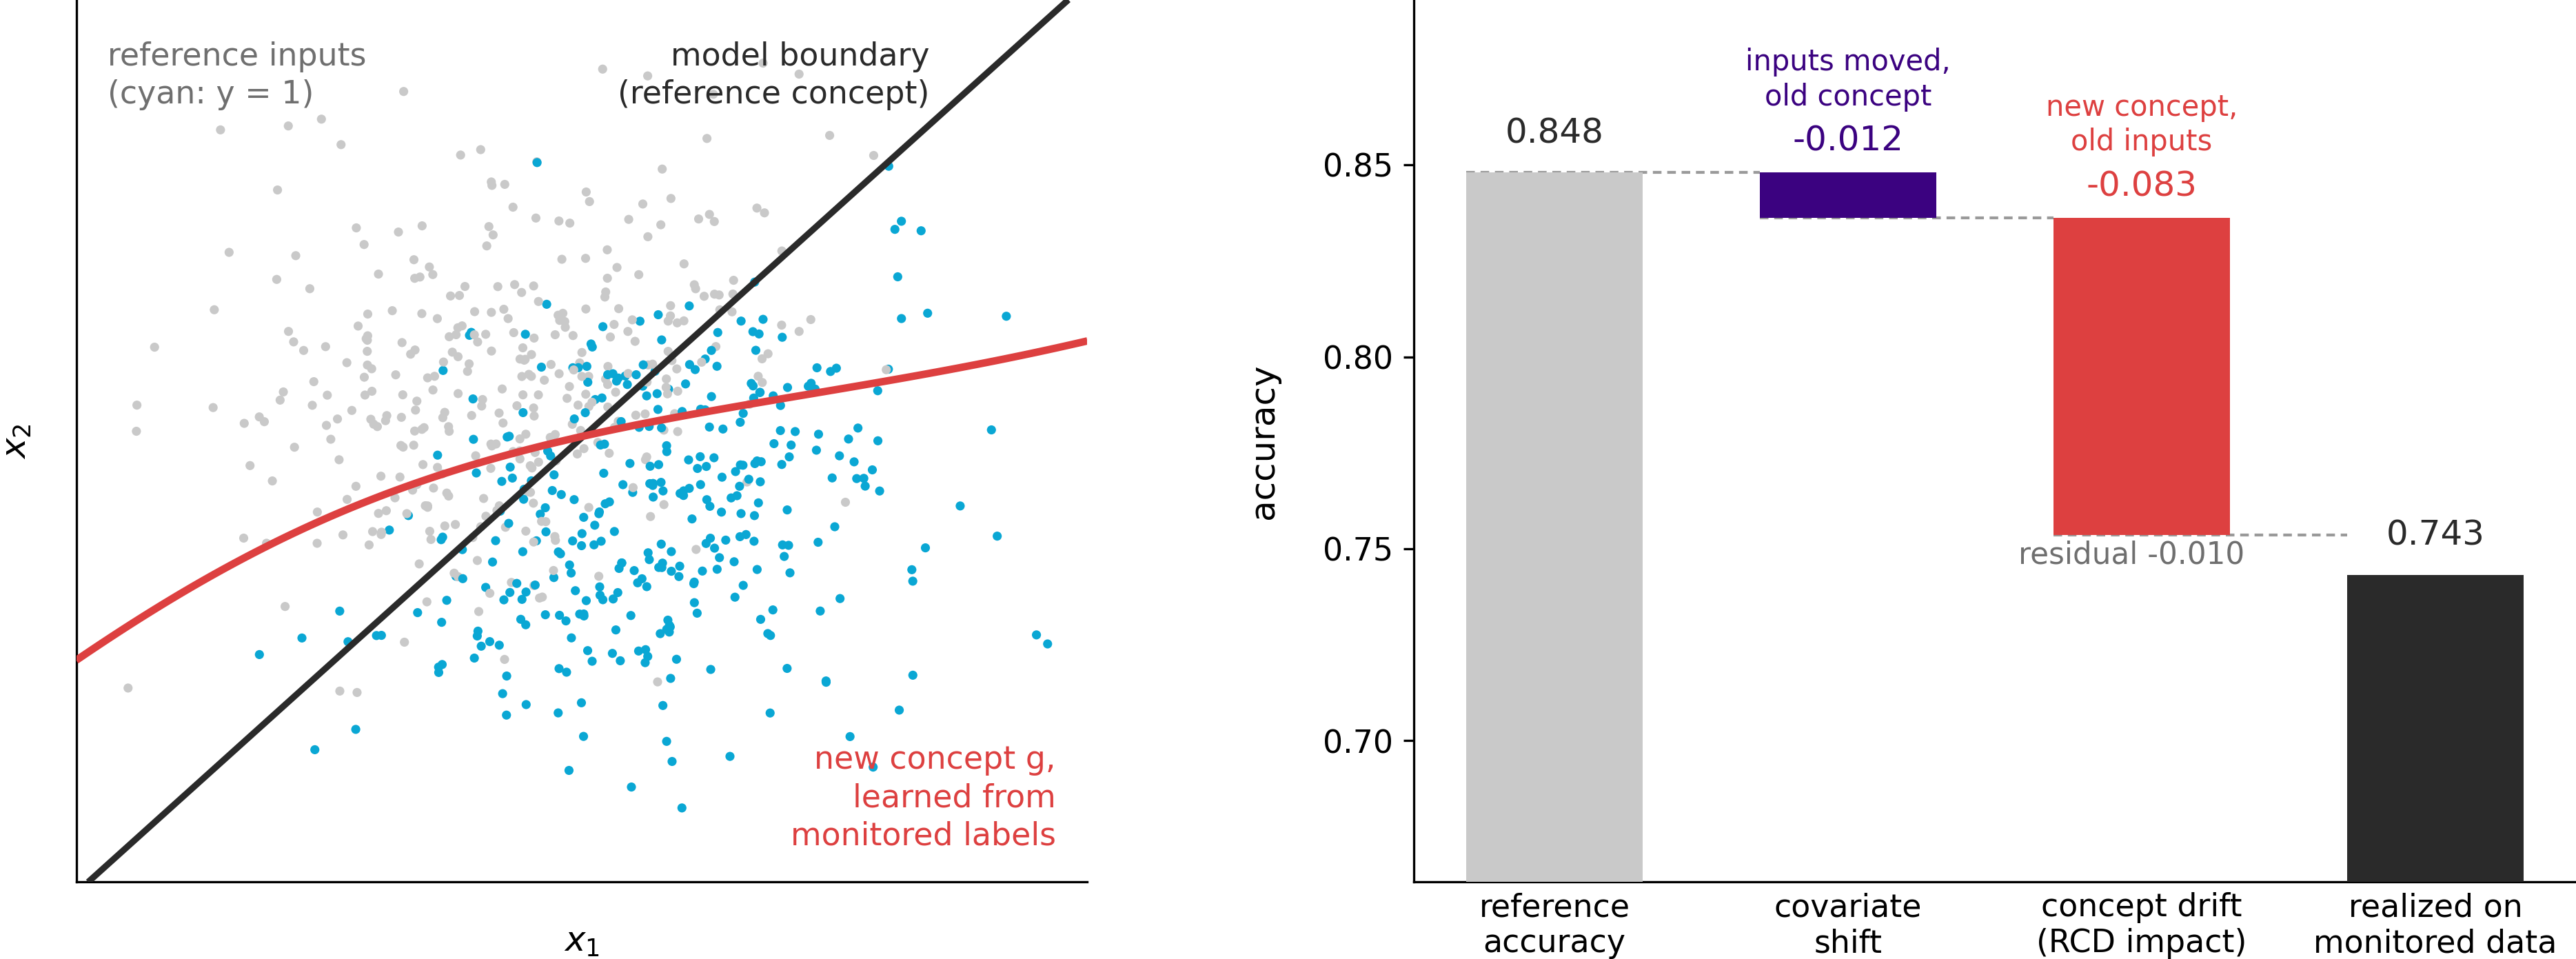
\includegraphics[width=\textwidth]{figures/RCD_decomposition.png}
\end{center}

\textbf{Figure. RCD.} \underline{Left:} simulated reference inputs, the monitored model's decision boundary (black), and the new
concept model's boundary (red). Between them, the models predict different classes. \underline{Right:} measured accuracy falls
from $0.832$ to $0.746$. Changing the input mix while keeping the old concept gives an estimated effect of $+0.010$; applying
the new concept to the reference inputs gives $-0.065$. These reach $0.777$, leaving a residual of $-0.031$. Interaction between
the shifts, concept-model error, and sampling variation can all contribute to that remainder.

\orangebox{Did you know that...}
{A large concept change can leave overall accuracy unchanged. Suppose a model predicts repayment for everyone in two equally
sized groups. Both groups initially repay $80\%$ of the time; later, one repays $100\%$ and the other $60\%$. Each rate changed
by twenty percentage points, but average accuracy is still $80\%$: the improvement in one group cancels the deterioration in
the other. A small overall impact can therefore hide a substantial change for particular groups.}

\textbf{Other related metrics}

CBPE, PAPE, and DLE assume the input--outcome relationship is stable; RCD helps investigate that assumption once labels arrive.
RCD also reports a \emph{magnitude}, $\frac{1}{n}\sum_j |g(x_j)-g_{\text{ref}}(x_j)|$, where $g_{\text{ref}}$ models the old concept
and the sum covers the reference inputs. This measures how much estimated probabilities changed, regardless of their effect on
accuracy. If magnitude is large but impact is small, examine individual groups for changes that cancel in the average.
